\documentclass[11pt]{article}

% packages
\usepackage[margin=0.85in]{geometry}
\usepackage{graphicx}
\usepackage{amsmath,amssymb}
\usepackage{booktabs}
\usepackage{xcolor}
\usepackage[hidelinks]{hyperref}
\usepackage[round]{natbib}
\usepackage[font=small,skip=4pt]{caption}
\usepackage{subcaption}

% formatting
\setlength{\parskip}{0.35em}
\setlength{\parindent}{0pt}
\renewcommand{\baselinestretch}{1.03}

% Pull the title block up so we don't waste an inch+ on whitespace.
\usepackage{titling}
\setlength{\droptitle}{-3em}
\posttitle{\par\end{center}\vskip 0.2em}

\title{
  Phase Reconstruction in a GAN-less Neural Audio Codec:\\
  A Failure-Mode Analysis and Rate-Distortion Study
}
\author{
  Ruiting Ma\\
  Master of AI, Monash University\\
  \texttt{rmaa0045@student.monash.edu}\\[0.4em]
  \small{Code: \url{https://github.com/RuitingMa/mini-codec}}
}
\date{}

\begin{document}
\maketitle

% =============================================================================
\begin{abstract}
\noindent
We implement an Encodec/SoundStream-style neural audio codec from
scratch and use it to characterise the failure modes of \emph{GAN-less}
training at low bitrate.
A 5.4M-parameter encoder, residual vector quantizer (RVQ), and decoder
are trained on \texttt{LibriSpeech train-clean-100} with a time-domain
$\ell_1$ plus multi-scale mel-spectrogram loss; no adversarial
discriminator is used.
On \texttt{test-clean} (256 utterances) at 3.2~kbps, per-sample
multi-scale mel-$\ell_1$ is tightly clustered (std~$\approx 0.009$)
while per-sample SI-SDR varies over a 30~dB range, identifying the
failure mode as phase / fine-time-structure error rather than
spectral envelope error.
A pre-registered ablation tests whether HuBERT-base layer-6 features
can substitute for adversarial training in supplying phase-aware
gradient: the additive variant is statistically indistinguishable from
the baseline on SI-SDR (median delta $-0.82$~dB at $\sim$1~dB SE),
while a swap-STFT control collapses to median $-30$~dB, together
ruling out HuBERT-style ASR-pretrained features as a phase-recovery
signal because they encode envelope but not phase.
A rate-distortion sweep at four bitrates ($1.6/3.2/6.4/12.8$~kbps,
all other parameters held fixed) yields a curve linear in
log-bitrate at $\sim$6~dB SI-SDR per octave, with the gap to
Encodec's published with-GAN numbers narrowing monotonically from
$\sim$21~dB at 1.6~kbps to $\sim$13~dB at 12.8~kbps, suggesting
the marginal contribution of adversarial training is largest where
the information bottleneck is tightest.
\end{abstract}

% =============================================================================
\section{Introduction}
\label{sec:intro}

Neural audio codecs based on encoder--quantizer--decoder pipelines
\citep{defossez2022high,zeghidour2021soundstream,kumar2023high} have
closed much of the perceptual quality gap to traditional codecs at
low bitrate. Their reported quality numbers depend, however, on a
multi-component loss that combines time-domain reconstruction,
multi-scale spectrogram losses, and an \emph{adversarial}
discriminator term in roughly equal weighting~\citep{defossez2022high}.
Removing the adversarial component is known empirically to lose
roughly $6$~dB of SI-SDR~\citep[\S3.5]{defossez2022high}, but the
mechanism behind that gap, and whether non-adversarial substitutes
could close it, is not well-characterised.

We therefore ask what a neural audio codec actually fails at when
trained without adversarial loss, and what class of substitute losses
could in principle replace adversarial training. Answering these
questions requires a setup that isolates the encoder, quantizer, and
reconstruction-loss design from the GAN dynamics, then probes those
choices systematically. We build that setup, a 5.4M-parameter
Encodec-style codec trained on \texttt{LibriSpeech}
\texttt{train-clean-100} with a deliberately GAN-free scope, and use
it to make three contributions.

The first is diagnostic. At the project's default 3.2~kbps operating
point, per-sample multi-scale Mel L1 across \texttt{test-clean} is
tightly clustered (std~$\approx 0.009$) while per-sample SI-SDR
ranges over 30~dB, identifying the residual error after non-adversarial
training as living in phase / fine-time-structure rather than in
spectral envelope (\S\ref{sec:failure}).
The second is a pre-registered ablation that asks whether features
from a frozen self-supervised audio encoder (HuBERT-base layer 6)
can supply the missing phase-aware gradient: an additive variant is
statistically indistinguishable from the baseline on SI-SDR
($\Delta = -0.82$~dB at SE $\sim 1$~dB), and a swap-STFT
anti-gaming control collapses to median $-30$~dB, ruling out a
structural family of perceptual losses for reasons we develop in
\S\ref{sec:perceptual}.
The third is quantitative: a four-point bitrate sweep at
$\{1.6, 3.2, 6.4, 12.8\}$~kbps yields a curve linear in log-bitrate
at $\sim 6$~dB SI-SDR per octave, with the gap to Encodec's
published with-GAN numbers narrowing monotonically from $\sim 21$~dB
at the low-bitrate end to $\sim 13$~dB at the high-bitrate end,
suggesting the marginal contribution of adversarial training is
largest where the information bottleneck is tightest
(\S\ref{sec:rd}).

% =============================================================================
\section{Method}
\label{sec:method}

\subsection{Architecture}
\label{sec:arch}

The encoder is a 1D convolutional stack with weight-normalised
\citep{salimans2016weight} \texttt{Conv1d} layers and ELU activations.
Downsampling factors $(2,4,5,5)$ give a $200\times$ temporal
compression, i.e.\ an 80~Hz frame rate at the project's 16~kHz native
sample rate; channel count doubles at each downsample; a final
$1\times 7$ projection emits a 128-dimensional latent. The decoder
mirrors the encoder using \texttt{ConvTranspose1d}, with
\texttt{output\_padding=1} on odd strides so the round-trip preserves
length to the sample. Compared to Encodec, the architecture trains
on the 16~kHz \texttt{train-clean-100} subset (rather than 24~kHz
mixed-domain data, so the encoder does not have to model music), uses
no LSTM bottleneck, and, as the central methodological choice for
this work, uses no adversarial discriminator. Total trainable
parameters: 5.4M, against Encodec's $\sim$14M.

\subsection{Quantizer}
\label{sec:rvq}

We use a residual vector quantizer (RVQ;~\citealp{zeghidour2021soundstream})
with 4 layers and 1024 codes per layer at the default bitrate point.
Codebooks are updated by EMA over assigned encoder outputs (no
autograd through them) and seeded data-dependently from the first
training batch.
We add a \emph{dual-trigger} dead-code restart that fires when either
(i) a code has gone $\geq 20$ consecutive steps without an assignment,
or (ii) its EMA cluster size has decayed below $0.01$.
The streak-based trigger is necessary at our scale: with batch~$\times$
segment frames~$=320$ and codebook size~$1024$, the steady-state EMA
cluster size for a uniformly used code is only $\sim$0.31, and an
EMA-only criterion at the canonical \citep{defossez2022high}
threshold of 2.0 would trigger continuously.
Without these stability tricks, all four RVQ layers collapse to a
single active code within $\sim$30 training steps.

\subsection{Loss}
\label{sec:loss}

The training objective for the baseline is a weighted sum of a
time-domain $\ell_1$ term, a multi-scale log-mel STFT term, and the
RVQ commitment loss:
\begin{equation}
\mathcal{L}
= 0.1 \cdot \Vert x - \hat x \Vert_1
+ \mathcal{L}_{\text{STFT}}
+ \mathcal{L}_{\text{commit}}.
\end{equation}
$\mathcal{L}_{\text{STFT}}$ is the multi-scale log-mel
$\ell_1+\ell_2$ distance over six STFT window sizes
$\{64,128,256,512,1024,2048\}$ (each scale with $\min(64, n_{\text{fft}}/8)$
mel bins, capped to keep the filterbank well-conditioned);
and $\mathcal{L}_{\text{commit}}$ is the standard RVQ commitment
loss \citep{vandenoord2017neural}. The perceptual ablation in
\S\ref{sec:perceptual} adds an optional fourth term
$\lambda \cdot \mathcal{L}_{\text{percep}}$. We use no adversarial
loss anywhere in this work: our project question is what
non-adversarial training can recover from this architecture, with
a within-architecture GAN ablation reserved as future work.

% =============================================================================
\section{Baseline failure mode}
\label{sec:failure}

The baseline is trained for 50k steps at batch size 16 with Adam
($\eta = 3\!\times\!10^{-4}$, $\beta = (0.9, 0.99)$) on a single
RTX 4090, taking roughly 35 minutes of wall time. Evaluation runs
on the first 256 utterances of \texttt{test-clean} with deterministic
crops and a fixed seed, scoring SI-SDR and the same multi-scale
Mel-$\ell_1$ used during training. At 3.2~kbps the baseline reaches
SI-SDR median $-14.10$~dB (std $10.35$~dB) and multi-scale Mel L1
median $0.309$ (std $0.215$). The standard deviation on SI-SDR is
driven largely by silence-dominated outliers, where SI-SDR is
sensitive to small reconstruction noise when the target is mostly
zero, so the median is the more representative summary statistic.

The two metrics' \emph{distributions} tell the more interesting
story. Per-sample multi-scale Mel-$\ell_1$ across the dumped subset
clusters tightly at std~$\approx 0.009$, while per-sample SI-SDR
spans 30~dB, three orders of magnitude apart in standard deviation.
Spectral envelope is reproduced with high consistency across
utterances; time-domain alignment is not. Inspection of the
per-sample spectrograms (Fig.~\ref{fig:spec}) confirms this directly.
Formant structure, energy distribution, and onset locations of the
input and the reconstruction match across the three variants we
plot, but the per-sample waveforms drift in phase by several
milliseconds even where the magnitude STFT is essentially identical.
This ``envelope reproduced, phase misaligned'' signature is
characteristic of GAN-less audio codecs at low bitrate.

\begin{figure}[t]
\centering
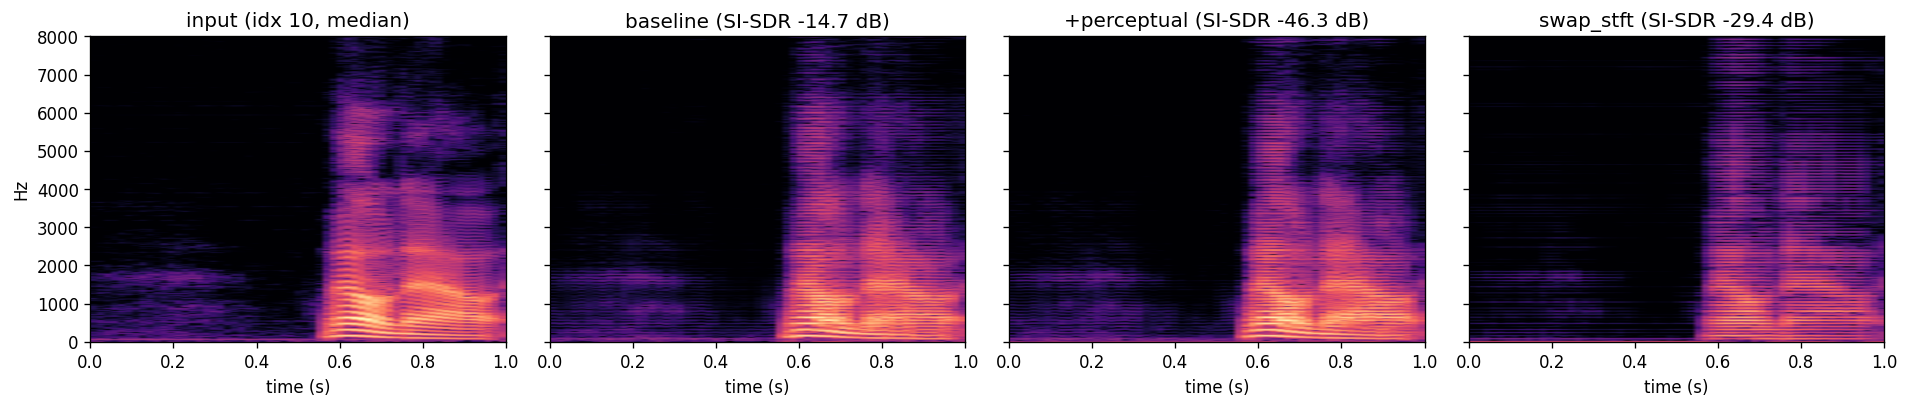
\includegraphics[width=0.9\linewidth]{figures/spectrogram_median.png}
\caption{Spectrogram comparison of the input and reconstructions
from baseline, additive perceptual, and swap-STFT variants on a
median-SI-SDR utterance from \texttt{test-clean}.
The envelope structure is preserved in baseline and \texttt{+perceptual}
even when their SI-SDR values differ by 30~dB; \texttt{swap\_stft}
has visible horizontal banding consistent with phase artefacts.
The median-rank utterance happened to be a \texttt{+perceptual}
catastrophic outlier (SI-SDR $-46.3$~dB); its envelope nevertheless
remains close to the input.}
\label{fig:spec}
\end{figure}

% =============================================================================
\section{Perceptual loss as a phase substitute? A pre-registered negative}
\label{sec:perceptual}

If a frozen pretrained self-supervised audio encoder produces
features whose stability requires phase information, then penalising
the $\ell_1$ distance between such features for $x$ and $\hat x$
should supply the codec with the phase-aware gradient that
time-domain L1 plus magnitude STFT does not provide. We test this
hypothesis with HuBERT-base \citep{hsu2021hubert} layer 6 features,
chosen as the standard phonetic / acoustic mid-layer after a
5k-step layer sweep over $\{4, 6, 9\}$.

The experiment uses two pre-registered conditions, recorded in the
project repository's experiment plan before training. The
\emph{additive} variant adds the perceptual term to the baseline
loss with weight 1.0; the \emph{swap-STFT} variant replaces the
multi-scale mel term with the perceptual term while leaving
everything else unchanged. The second variant is an anti-gaming
control. If perceptual loss alone is too weak to support codec
training, swap-STFT will collapse; if perceptual loss is
independently strong, swap-STFT should match or exceed the
baseline. Without this control, an additive variant that improves
on baseline could equally well be reading off the STFT term that
already does most of the work.

Results on the same 256-utterance \texttt{test-clean} pass appear
in Table~\ref{tab:perceptual}. The additive variant reaches median
SI-SDR $-14.92$~dB, a $0.82$~dB drop relative to baseline at a
standard error of roughly $1$~dB, well within the pre-registered
``failed'' threshold of a $1$~dB lift in either direction. Mel L1
marginally improves (0.301 vs.\ 0.309), the only metric that moves
systematically in the positive direction. The swap-STFT variant
collapses to median SI-SDR $-30.12$~dB, a $16$~dB regression from
baseline at which the model is essentially producing noise.

\begin{table}[t]
\centering
\caption{HuBERT-base layer-6 perceptual loss vs.~baseline,
\texttt{test-clean} 256 utterances.}
\label{tab:perceptual}
\begin{tabular}{lcccc}
\toprule
Variant & SI-SDR median (dB) & SI-SDR mean (dB) & Mel L1 median & Mel L1 mean \\
\midrule
baseline & $-14.10$ & $-15.70$ & 0.309 & 0.399 \\
{}+perceptual (additive) & $-14.92$ & $-16.05$ & \textbf{0.301} & \textbf{0.396} \\
swap-STFT & $-30.12$ & $-32.04$ & 0.693 & 0.864 \\
\bottomrule
\end{tabular}
\end{table}

Read together, the two conditions rule out the most charitable
interpretation of the additive result. If the perceptual loss were
contributing useful phase signal that the STFT term simply absorbs,
swap-STFT, where there is no STFT to absorb anything, should still
train at least to baseline-level reconstruction quality. It does not.
The perceptual loss is therefore not independently strong enough to
replace STFT's spectral signal, and the additive variant's small
Mel-$\ell_1$ improvement (with no SI-SDR change) places HuBERT's
contribution in exactly the spectral envelope dimension that
multi-scale STFT already covers. We argue the cause is structural.
HuBERT and similar SSL audio encoders are trained on masked-prediction
objectives that can be satisfied using envelope / phonetic content
alone; their representations need not encode phase, and our results
suggest they in fact do not. A perceptual loss derived from such an
encoder cannot supply phase-aware gradient regardless of layer
choice, which closes off this entire family of substitutes for
adversarial training.

% =============================================================================
\section{Rate-distortion characterisation}
\label{sec:rd}

To characterise the codec's capacity at the chosen architecture, we
sweep the number of RVQ layers
$N \in \{2, 4, 8, 16\}$, holding everything else fixed.
The resulting bitrates are $\{1.6, 3.2, 6.4, 12.8\}$~kbps. Each
configuration is trained from scratch for 50k steps; evaluation is
the same 256-utterance \texttt{test-clean} pass.

The resulting rate-distortion curve in Fig.~\ref{fig:rd} is
approximately linear in log-bitrate, with per-octave SI-SDR gains
of $5.93$, $7.47$, and $5.68$~dB across the three intervals. Higher
bitrates also produce more consistent reconstructions: the
inter-quartile range narrows monotonically from $12.5$~dB at
$1.6$~kbps to $8.2$~dB at $12.8$~kbps. Per-sample improvements are
universal as well: Fig.~\ref{fig:rd_delta} shows that the SI-SDR
delta from $1.6$ to $12.8$~kbps is entirely positive across the 256
utterances (median $+19.4$~dB, range roughly $+3$ to $+60$~dB). No
sample regresses with more bits, so the bitrate increase is being
spent productively across the full distribution rather than fitting
a few easy samples.

Comparison to Encodec's published numbers~\citep[Table 4]{defossez2022high}
is informative even though our setup is not a controlled ablation
of theirs. The gap is $\{21.5, 18.6, 15.1, 13.0\}$~dB at the four
bitrates, a monotonic narrowing of $8.5$~dB across the sweep.
Encodec's setup differs from ours in several respects (adversarial
loss, 24~kHz mixed-domain training data, a larger model, and a much
larger training corpus), so we cannot read this trend as a clean
measurement of the GAN contribution. Since adversarial training is,
however, the most distinctive methodological difference between the
two systems, the narrowing is consistent with the hypothesis that
GAN's marginal contribution to perceptual quality is largest where
the information bottleneck is tightest. Adversarial training is the
mechanism best positioned to ``fill in'' detail the encoder
physically cannot store; at $12.8$~kbps, where the encoder has
enough bits to encode that detail directly, the marginal value of
the discriminator should plausibly be smaller.

An informal listening check by the author on a handful of
$12.8$~kbps reconstructions matched the metric picture: speech is
fully intelligible and the spectral envelope is recognisable, while
residual phase and timbre artefacts remain clearly audible. This is
consistent with the codec sitting at SI-SDR $\approx 0$~dB: good
enough that the signal is recovered, not good enough that the
reconstruction is transparent. A formal listening study is left
to future work.

\begin{figure}[t]
\centering
\begin{subfigure}[t]{0.49\linewidth}
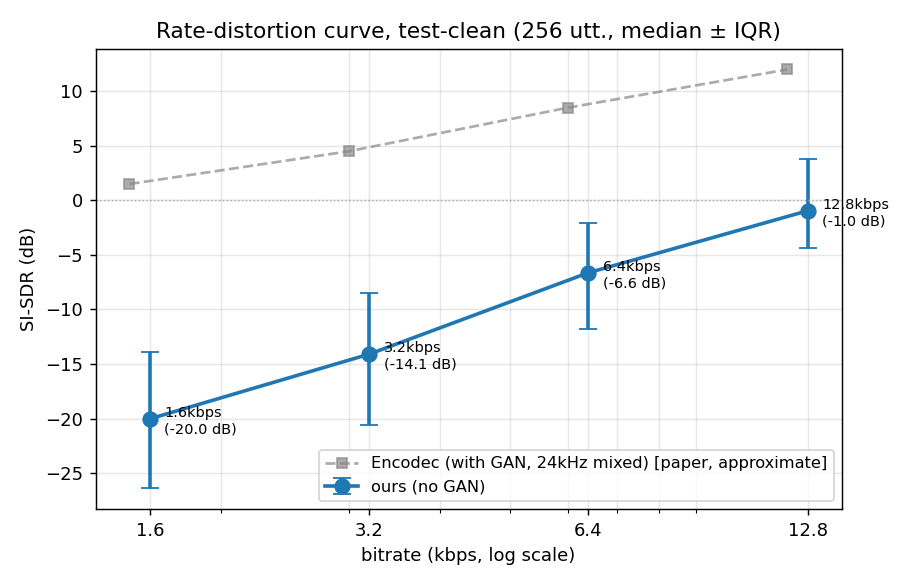
\includegraphics[width=\linewidth]{figures/rd_curve.png}
\caption{R-D curve: SI-SDR median ($\pm$IQR) vs.~bitrate. Encodec
reference is approximate, from the paper's Table 4 (24~kHz mixed,
with GAN); see text for caveats.}
\label{fig:rd}
\end{subfigure}\hfill
\begin{subfigure}[t]{0.49\linewidth}
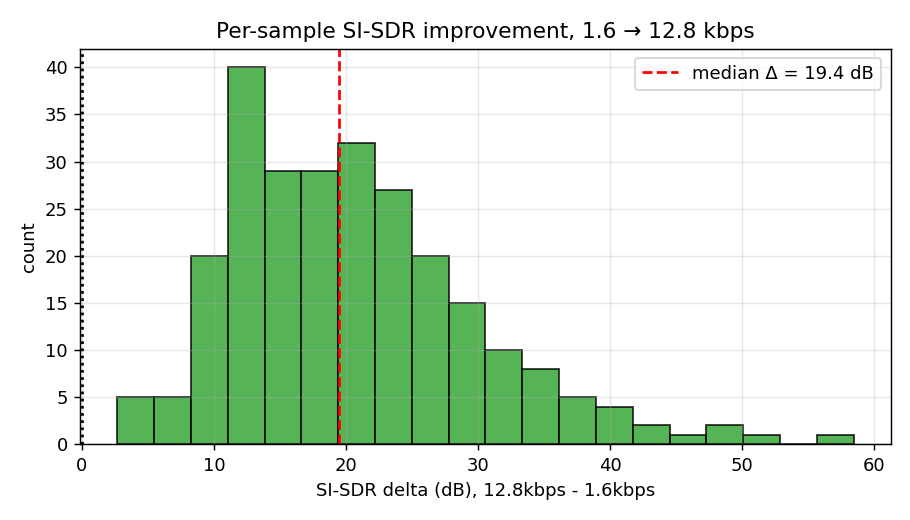
\includegraphics[width=\linewidth]{figures/per_sample_delta.png}
\caption{Per-sample SI-SDR delta, 12.8~kbps minus 1.6~kbps. Every
utterance improves; median $+19.4$~dB.}
\label{fig:rd_delta}
\end{subfigure}
\caption{Rate-distortion behaviour of the codec at fixed architecture.}
\end{figure}

% =============================================================================
\section{Discussion}

Our codec at $12.8$~kbps reaches a median SI-SDR of $-1.0$~dB,
the first bitrate at which target-signal energy and reconstruction-
error energy are roughly comparable. The gap to Encodec at
$1.6$~kbps is around $22$~dB and at $12.8$~kbps around $13$~dB,
larger in both cases than the $\sim 6$~dB Encodec itself attributes
to adversarial training in their own
ablation~\citep[\S3.5]{defossez2022high}. The residual several dB
across the curve presumably reflect the other differences in data,
scale, and architecture detail. Within our own setup, the
gap-narrowing trend is the more interesting object than the absolute
size of the gap, because it is internally consistent: the same
codec evaluated under the same protocol approaches the with-GAN
reference more closely as the bottleneck loosens.

A complementary view of the perceptual-loss negative result links
this back to \S\ref{sec:perceptual}. The swap-STFT collapse is a
clean falsification: in a setting where the perceptual loss is the
only spectral signal available to the model, training fails to
reach even baseline-level reconstruction. The additive variant's
near-equivalence to baseline therefore cannot be attributed to
``perceptual is doing the work that STFT used to do''. The
perceptual loss is simply weaker than STFT in the envelope
dimension and provides nothing in the phase dimension, leaving the
codec with the same gradient signal it had before.

The cleanest experimental follow-up is a within-architecture GAN
ablation, which would let us decompose the gap-narrowing trend in
Fig.~\ref{fig:rd} into a controlled adversarial contribution and the
residual data / scale / architecture confound. The conceptually
deeper question, raised by the structural argument in
\S\ref{sec:perceptual}, is whether a \emph{phase-aware}
self-supervised audio encoder is achievable as a pretraining target.
Our HuBERT result identifies the gap negatively; constructing
pretext tasks whose representations must encode phase, and
evaluating the resulting features as a non-adversarial perceptual
loss, is an open problem we believe is worth its own line of work.

% =============================================================================
\section{Limitations and future work}
\label{sec:future}

Several limitations qualify the conclusions above. The most
significant is that we use no adversarial discriminator, by design,
which caps how strong the absolute SI-SDR numbers from this
architecture can be and means the bitrate-scan curve sits below
any system that does use one. Each bitrate point is also a single
seed and a single training run, so we have no within-condition
variance estimates against which to gauge the per-octave gain we
report. Evaluation is on speech alone; generalisation to music is
not characterised. Finally, the Encodec reference numbers in
Fig.~\ref{fig:rd} are read approximately from a published table
on a different setup (different sample rate, training corpus, and
model size), so the gap-narrowing trend in our comparison can only
be motivated, not concluded, until the controlled within-architecture
ablation we propose below has been run.

The most direct experimental follow-up is precisely that controlled
GAN ablation: training the same architecture with and without an
adversarial discriminator at all four bitrates would let us
decompose the gap-narrowing trend into a clean adversarial
contribution and a residual confound. Beyond that, our HuBERT
negative result motivates a longer-horizon question: whether a
self-supervised pretraining objective can be designed so that the
resulting representations must encode phase information, providing
a non-adversarial path to the phase signal that this work has shown
ASR-style SSL features cannot supply. Smaller follow-ups also
suggest themselves. Quantizer dropout~\citep{zeghidour2021soundstream}
would let a single trained model support multiple inference
bitrates rather than the four independent models we trained here.
Phase-specific differentiable losses such as instantaneous
frequency or group-delay distortion are an alternative to
adversarial training that does not require a discriminator network.
And evaluation on a music-domain dataset would characterise the
codec's transfer behaviour beyond clean read speech.

% =============================================================================
{\small
\setlength{\bibsep}{0.15em plus 0.1em}
\bibliographystyle{abbrvnat}
\bibliography{refs}
}

\end{document}
